

\subsection{Kinetic phase transfer NAPL - water}

In this benchmark, a simplified two-phase (NAPL-water) flow model is coupled with mass transport and kinetic dissolution of the NAPL phase. The NAPL here is assumed to be in residual saturation and hence immobile, while the water phase is mobile and transports the dissolved species. The PS\_GLOBAL model is used for the simulation of the two-phase flow process. Two simple tests first are used to verify the correctness of the flow field and the coupling of flow and transport processes for all element types. The kinetic dissolution model is tested by comparison to an analytical solution.

\subsubsection{Flow in presence of a residual immobile NAPL phase}
\label{NAPL_diss_BM_flow}

Groundwater flow in presence of a residual NAPL phase is simulated in a one-dimensional model of 50 m length in $x$ direction. The residual NAPL is present as blobs (or ganglia) in a five m long zone between $x$ = 5 - 10 m from the left hand side boundary of the model and has a saturation $S_n$ = 0.10. Accordingly, water saturation $S_w$ = 0.90 in this zone, while $S_w$ = 1.0 elsewhere. Water phase relative permeability $k_{r_w}$ [-] is described using the Brooks-Corey model
\begin{equation}
k_r = \left(S_{eff}\right)^{\frac{2+3\lambda}{\lambda}}
\label{eq_brooks-corey_krel}
\end{equation}
with $\lambda$ $= 0.386$ [-] as an empirical parameter, and is reduced to a value of 0.625 in the NAPL zone. Water effective saturation is given by
\begin{equation}
S_{eff} = \frac{S_w-S_{r_w}}{S_{s_w}-S_{r_w}}
\label{eq_Seff_brooks-corey}
\end{equation}
NAPL immobility is achieved by setting the NAPL residual saturation $S_{r_n} > S_n$. NAPL phase relative permeability accordingly is 0.0 throughout the model domain.

As the NAPL is in residual saturation and thus immobile, and dissolution reactions are not considered at the moment, $S_n$, $S_w$ and $k_{r_w}$ remain temporally constant. Constant pressure boundary conditions are used on the left and right hand side model boundary, which induce an average hydraulic gradient of 0.01. Linear, quadrilateral, hexahedral, triangular, prismatic as well as tetrahedral elements are used for the spatial discretization of the model. The size of the elements is 1/3 m in $x$ direction in each case, i.e. for the 1D line element model, 150 elements are used. Model parameters for the simulation are summarized in Tab.~\ref{l_tab_benchmark_1d_NAPLdiss_hydr}.

\begin{table}[htbp]
\caption{Model parameters used for the test case. }
\centering
\begin{tabular}{|l|l|l|}
\hline
parameter & value & unit \\
\hline
model length $x$ &	50	& m  \\			
\hline
model length $y$ &	1.0	& m  \\		
\hline
model length $z$ &	1.0	& m  \\		
\hline
element length $x$ &	0.333	& m  \\		
\hline
porosity $n$  & 0.25 &  --  \\			
\hline
permeability $k$  & 1.54249$\cdot$10$^{-11}$ &  m$^2$  \\			
\hline
tortuosity $\tau$ & 1.0  & -- \\
\hline
residual water saturation $S_{r_w}$ & 0.2 & -- \\
\hline
saturated water saturation $S_{s_w}$ & 1.0 & -- \\
\hline
residual NAPL saturation $S_{r_n}$ & 0.2 & -- \\
\hline
saturated NAPL saturation $S_{s_n}$ & 0.95 & -- \\
\hline
$\lambda$ (Brooks-Corey parameter) & 3.86 & -- \\
\hline
density of water $\rho_w$ & 1000 & kg  m$^{-3}$ \\
\hline
viscosity water $\eta$ & 0.001 & Pa s \\
\hline
initial $S_w$ ($x<$5 m \& $x>$10 m, $t$=0)  & 1.0 & -- \\
\hline
initial $S_w$ ($x>$5 m \& $x<$10 m, $t$=0)  & 0.90 & -- \\
\hline
initial $S_n$ ($x<$5 m \& $x>$10 m, $t$=0)  & 0.0 & -- \\
\hline
initial $S_n$ ($x>$5 m \& $x<$10 m, $t$=0)  & 0.10 & -- \\
\hline
initial water pressure ($x$, $t$=0) & 98067.0  & Pa \\
\hline
water pressure ($x$=0, $t$) &  98067.0 & Pa \\
\hline
water pressure ($x$=50, $t$) & 93163.65 & Pa \\
\hline
\end{tabular}
\label{l_tab_benchmark_1d_NAPLdiss_hydr}
\end{table}

The hydraulic 1D model is compared against an equivalent single (water) phase groundwater flow model, in which a zone of reduced hydraulic permeability is introduced at the position of the NAPL zone (i.e. between $x$ = 5 m and $x$ = 10 m), with $K$ = 9.64056$\cdot10^{-12}$ m$^2$, which corresponds to $K$ in the NAPL zone of the two-phase model.

Fig.~\ref{profiles_pressure_NAPLflow} shows the numerical solution of the pressure distribution after a time step of 21600 s. The pressure gradient in the water phase is uniform up to $x$ = 5 m, increases in the NAPL zone due to the reduction of permeability and decreases again for $x>$ 10 m. Simulations for all element types show identical pressure distributions. The individual graphs therefore cannot be distinguished in Fig.~\ref{profiles_pressure_NAPLflow}.

\begin{figure}[htbp]
\centering
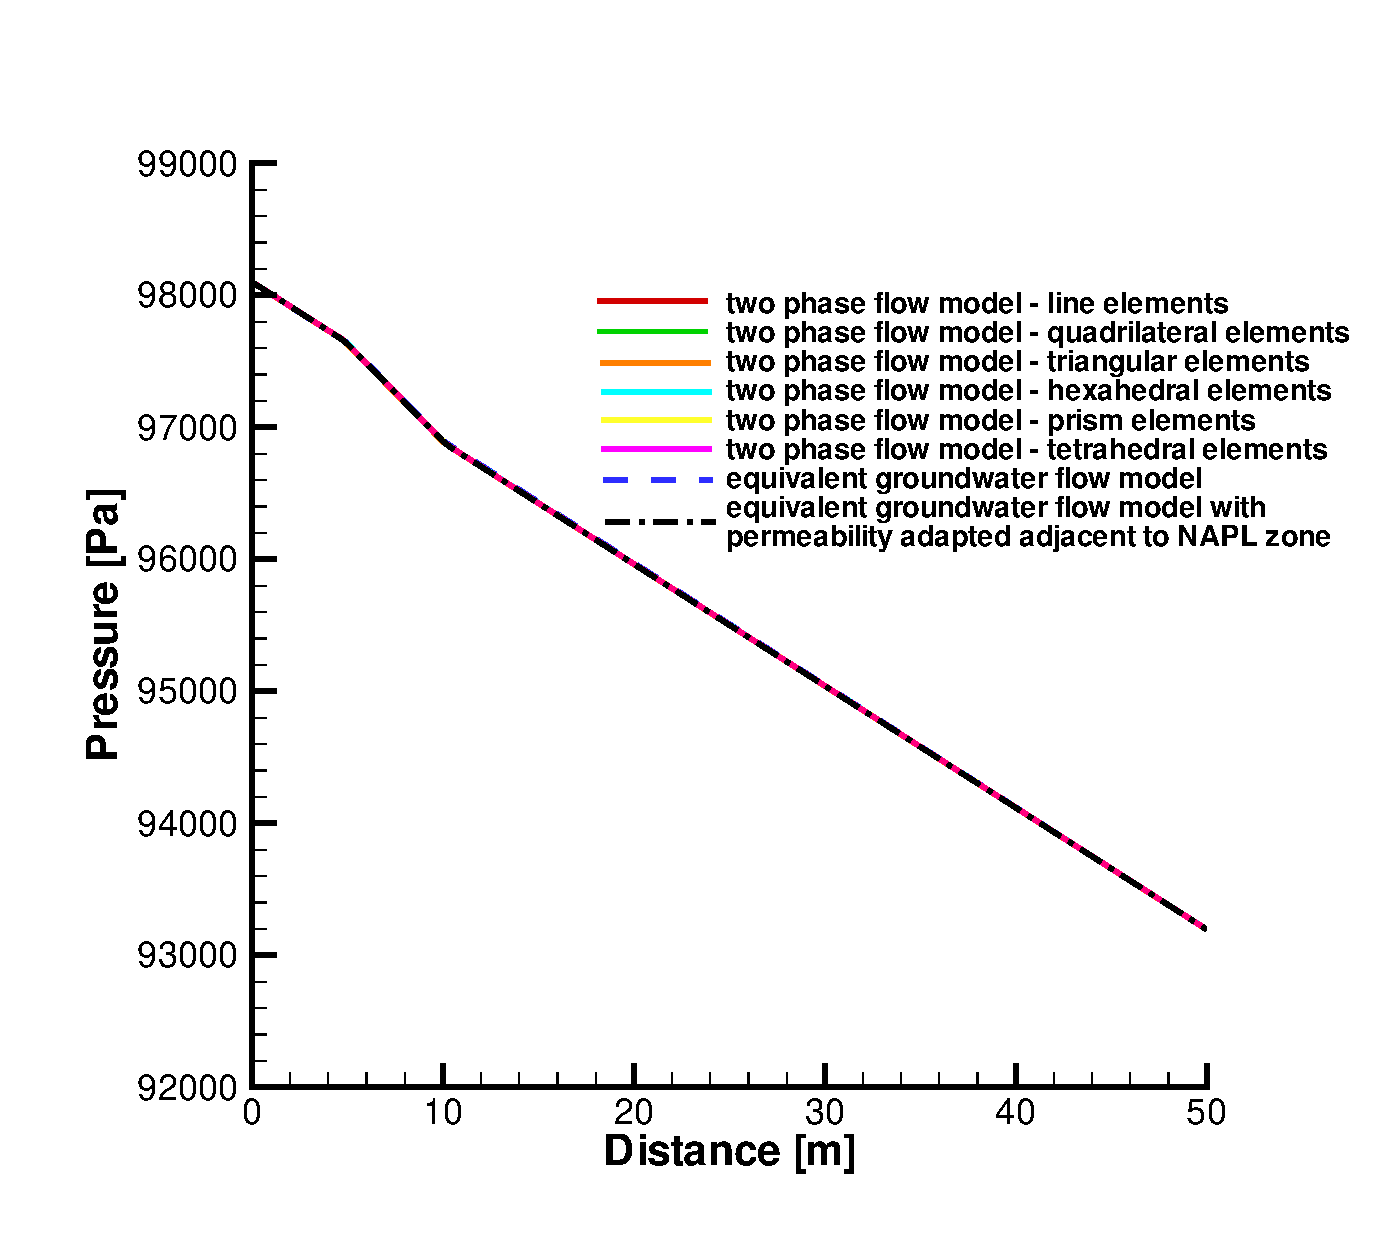
\includegraphics[width=0.6\textwidth]{C/figures/NAPL_diss_pressure.eps}
\caption{Water phase pressure distribution along the 1D model for different element types and two equivalent single phase groundwater flow models with reduced hydraulic permeability between $x$ = 5 m and $x$ = 10 m.}
\label{profiles_pressure_NAPLflow}
\end{figure}

The pressure distribution of the groundwater flow model (blue dashed graph) matches the two-phase model pressure distribution almost exactly, although some very small discrepancies exist at the transition zones between NAPL zone and the fully water saturated domain. These differences are due to the handling of the discontinuous phase saturation distribution at the boundaries of the NAPL zone, i.e. at $x$ = 5 and $x$ = 10 m. In the two-phase model, for elements in the direct vicinity of the NAPL zone element matrices are calculated assuming a saturation interpolated from the element nodes saturation values, which results in $S_n >$ 0, $S_w <$ 1 and $k_{r_w} <$ 1, and the observed deviation from the pressure distribution of the groundwater flow model. In Fig.~\ref{profiles_pressure_NAPLflow} the black dash-dotted graph shows the pressure distribution from a modified groundwater flow model, where a hydraulic permeability of $K$ = 1.229174$\cdot10^{-11}$ m$^2$ was assigned to the two elements in the direct vicinity of the NAPL zone, which corresponds to the reduced water phase permeability of these elements in the two-phase model. In this case the pressure distribution matches the two-phase model results exactly.

\subsubsection{Conservative transport in presence of a residual immobile NAPL phase}
\label{NAPL_diss_BM_transport}

This test is based on the previously presented simulation, which is extended for a conservative mass transport process by infiltration of a non-reactive tracer at a constant concentration of 1.0 at the left hand side model boundary, i.e. at $x$ = 0 m, for a period of 500 time steps of 21600 s. Longitudinal dispersivity  $\alpha_L$ = 0.5 m, the aqueous diffusion coefficient D$_{aq}$ = 1$\cdot10^{-9}$ m$^2$ s$^{-1}$. All other model parameters are kept identical to the previous test case.

In contrast to transport in fully water saturated media, in the presence of a NAPL phase transport takes place in a reduced volume $nS_w$, where $S_w$ is taken from the flow step (and hence from the old time level)
\begin{equation}
    n S_w\frac{\partial C_{w,i}}{\partial t} + \textbf{\textrm{q}}_w \nabla C_{w,i} - \nabla \cdot\left( nS_w\textbf{\textrm{D}}_i \nabla C_{w,i} \right)+nS_wQ_{C_{w,i}}=0
    \label{eq_trans_water_NAPLdiss}
\end{equation}
where $C_{w,i}$  [M L$^{-3}_{water}$] is the concentration of component $i$ in groundwater, \textbf{q}$_w$ the Darcy velocity [L T$^{-1}$] and \textbf{D}$_i$ the dispersion tensor [L$^2$T$^{-1}$]. As the NAPL phase is stationary and residual, its phase velocity is zero and components present in the NAPL phase remain immobile. The corresponding transport equation hence only consists of the source term from NAPL dissolution:
\begin{equation}
    n S_n\frac{\partial C_{w,j,i}}{\partial t} +nS_nQ_{C_{n,j,i}}=0
    \label{eq_trans_NAPL_NAPLdiss}
\end{equation}
As the source term in \ref{eq_trans_NAPL_NAPLdiss} is explicitly accounted for in the computation of the exchange processes (see below), a solution of \ref{eq_trans_NAPL_NAPLdiss} on the model grid is not necessary.

The 1D transport model is compared against an equivalent single (water) phase groundwater flow and transport model. Fig.~\ref{profiles_tracer_NAPLtransp} presents breakthrough curves of the tracer at $x$ = 15 m, i.e. 5 m downgradient from the NAPL zone, for all element types and the two equivalent groundwater flow models, in which in addition to the permeabilities also porosities were matched with the effective porosities of the two-phase model. Results for all element types compare well, although a plot of breakthrough concentrations on a logarithmic scale (right diagram) reveals small differences between different element types for early moments of the two-phase simulation and small breakthrough concentrations. In comparison, the tracer breakthrough curve for the equivalent groundwater flow model matches the results of the two-phase model precisely.

\begin{figure}[htbp]
\centering
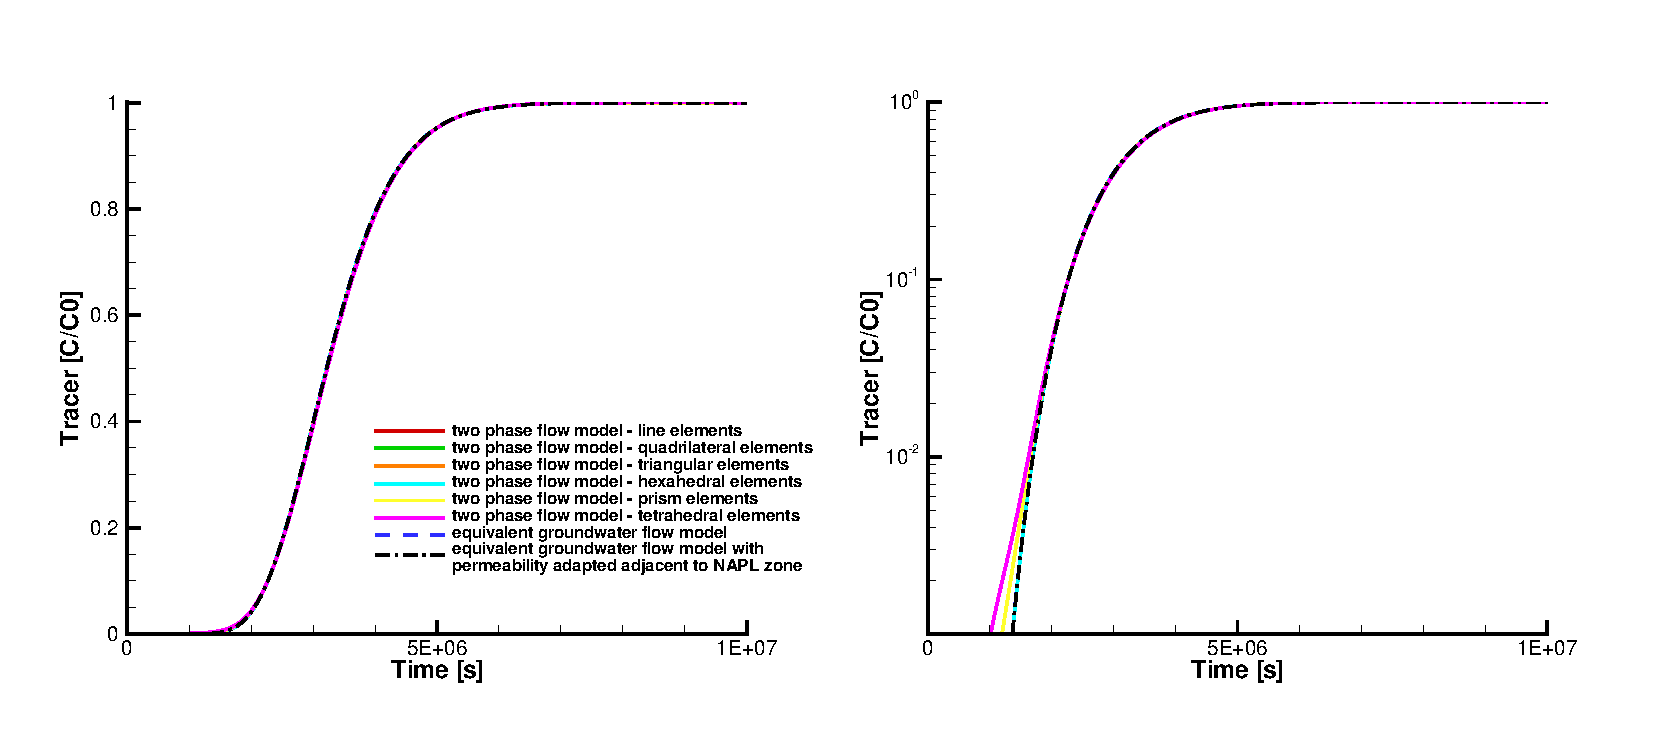
\includegraphics[width=1\textwidth]{C/figures/NAPL_diss_BTC.eps}
\caption{Tracer breakthrough concentrations in the 1D model at $x$ = 15 m downgradient from the left hand side model boundary for different element types and two equivalent single phase groundwater flow models with reduced hydraulic permeability between $x$ = 5 m and $x$ = 10 m. Left diagram: linearly scaled concentrations; right diagram: logarithmic concentrations.}
\label{profiles_tracer_NAPLtransp}
\end{figure}


\subsubsection{Dissolution of a multi-component NAPL phase}
\label{NAPL_diss_BM_diss}

The kinetic dissolution model is validated against the Hansen and Kueper analytical solution ~\cite{HanKue:07}. The  Hansen and Kueper model ~\cite{HanKue:07} model was developed to quantify the temporally changing composition of a residual multi-component NAPL body in moving groundwater and the consequent changes of the NAPL constituents concentrations in the surrounding groundwater. It is suited for both, pooled configurations and residual NAPL in blob geometries and - as any analytical model - is based on a number of simplifying assumptions:
\newenvironment{bulletpopints}{\begin{itemize}}{\end{itemize}}
\begin{bulletpopints}
 \item The model predicts the NAPL composition as well as aqueous phase concentrations at the downstream end of the NAPL source zone (Fig.~\ref{fig_HKAS_concept}).
\item  Intra-NAPL diffusion is fast in relation to phase partitioning.
\item  For pools the local equilibrium assumption is employed, i.e. inter-phase mass transfer is faster than solute transport away from the NAPL.
\item  Within a zone of residual NAPL, NAPL saturation and mixing are sufficient to allow the assumption of a uniform concentration composition at the downstream end of the source zone (perfectly mixed source), which follows Raoult's law (global equilibrium assumption).
\item  The component composition of the NAPL is spatially invariant at a particular instant in time.
\item  Dissolution kinetics are fast at all times (equilibrium dissolution).
\item  NAPL saturation, effective porosity and water flux through the source are constant in time.
\end{bulletpopints}

The Hansen and Kueper model ~\cite{HanKue:07} for a residual NAPL source zone was represented as a one-dimensional numerical model of 50 m length in $x$ direction using linear finite elements and a spatial discretization $\Delta x$ = 1/3 m, i.e. the same model geometry as in the previous two test cases is used here. The assumption of a perfectly mixed residual NAPL source zone is represented as a zone of blobs at a single node of the finite element mesh directly downgradient of the left hand side model boundary at $x$ = 1/3 m (Fig.~\ref{fig_HKAS_FEM}).

\begin{figure}[htbp]
\centering
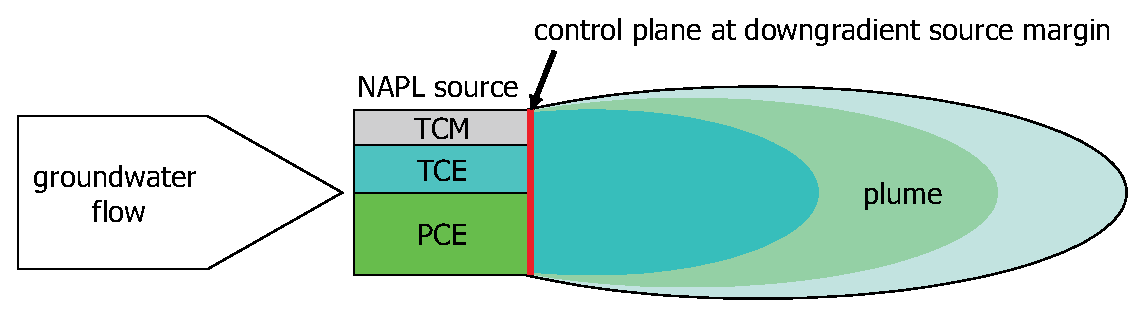
\includegraphics[width=0.9\textwidth]{C/figures/H&K_concept.eps}
\caption{Conceptualization of the Hansen and Kueper (2007) analytical solution: Example of a three component residual NAPL source zone in a moving groundwater body and source emission.}
\label{fig_HKAS_concept}
\end{figure}

\begin{figure}[htbp]
\centering
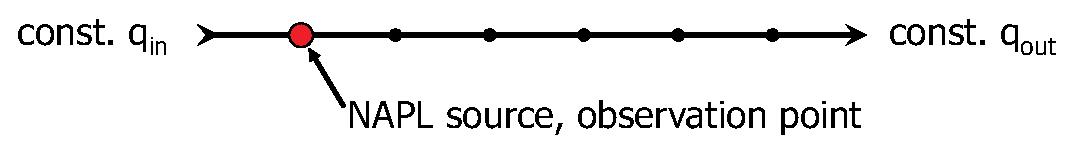
\includegraphics[width=0.9\textwidth]{C/figures/H&K_concept_FEM.eps}
\caption{Representation of the Hansen and Kueper (2007) analytical solution in a numerical model. The red dot represents the position of the NAPL blob zone in the linear finite element mesh.}
\label{fig_HKAS_FEM}
\end{figure}

The temporally constant flux through the NAPL source is induced by source terms of $q_{in} =-q_{out} = 1.157\cdot10^{-6}$ m s$^{-1}$ at the left and right hand side model boundaries, respectively (Fig.~\ref{fig_HKAS_FEM}). The NAPL consists of the three chlorinated hydrocarbon (CHC) species perchloroethene (PCE), trichloroethene (TCE) and tetrachloromethane (TCM). Accordingly, three immobile NAPL species plus three corresponding mobile species are defined in the model. Tab.~\ref{l_tab_benchmark_1d_HKAS_compprop} lists physicochemical parameters and initial amounts or concentrations, respectively, assumed for the three immobile NAPL species in this simulation.

\begin{table}[htbp]
\caption{Physicochemical properties and initial concentrations of the immobile NAPL species.}
\centering
\begin{tabular}{|l|l|l|l|l|}
\hline
parameter & Unit & PCE & TCE & TCM \\
\hline
molar weight & [kg mol$^{-1}$] & 0.166 & 0.131 & 0.154	\\
\hline
molar density & [mol m$^{3}$] & 9770.800 & 11111.100 & 12395.300\\	
\hline
max. aq. solubility & [mol/m$^{3}$] & 1.150 & 10.650 & 72.860\\
\hline
concentration & [mol/m$^{3}_{REV}$] & 122.140 & 111.110 & 30.990\\
\hline
volume per m$^{3}_{REV}$ & [m$^3$] & 0.013 & 0.010 & 0.003\\
\hline
mass per m$^{3}_{REV}$ & [kg] & 20.254 & 14.599 & 4.767\\
\hline
\end{tabular}
\label{l_tab_benchmark_1d_HKAS_compprop}
\end{table}

Corresponding mobile species in the aqueous phase share the same physicochemical properties. Initial concentrations at the second node of the mesh (i.e. at the NAPL source position) correspond the equilibrium concentrations according to Raoult's law and the initial moles of the immobile NAPL components, i.e. C$_{PCE}$ = 0.532, C$_{TCE}$ = 4.478 and C$_{TCM}$ = 8.545 mol m$^{-3}$, respectively. Elsewhere, initial concentrations (as well as upstream boundary conditions) are set to C = 1.0$\cdot10^{-10}$ mol m$^{-3}$. In the NAPL source S$_n$ = 0.10 and S$_w$ = 0.90, accordingly, while S$_w$ = 1.0 and S$_n$ = 0.0 elsewhere. Water phase relative permeability k${_{r_w}}$ [-] is described by the Brooks-Corey model (see above). Other model parameters (and those deviating from the model setup of the previous two test cases) are summarized in Tab.~\ref{l_tab_benchmark_1d_HKAS_hydr}.

\begin{table}[htbp]
\caption{Model parameters used for benchmark ~\ref{NAPL_diss_BM_diss} }
\centering
\begin{tabular}{|l|l|l|}
\hline
parameter & value & unit \\
\hline
longitudinal dispersivity  $\alpha_L$  & 0.09 &  m\\
\hline
mean grain diameter $d_{50}$  & 0.001 &  m\\
\hline
Sherwood factor $SF$  & 1.15 &  --\\
\hline
Reynolds exponent $RE$  & 0.654 &  --\\
\hline
Schmidt exponent $SE$  & 0.486 &  --\\
\hline
interfacial area $a$  & 5000.0 &  m$^2$ m$^{-3}_{REV}$\\
\hline
\end{tabular}
\label{l_tab_benchmark_1d_HKAS_hydr}
\end{table}



Mass transfer between the NAPL and the aqueous phase for individual components $i$ is described by Fick's 1st law
\begin{equation}
    \frac{\partial M}{\partial t} =  k a \left( C_{w,i}^{sat}  -  C_{w,i}  \right)
    \label{eq_mass_transfer}
\end{equation}
The rate of mass transfer [M T$^{-1}$] depends mainly on the concentration difference between the equilibrium concentration [M L$^{-3}$] and the actual concentration [M L$^{-3}$] in the water phase as well as on the mass transfer parameter $k$ [L T$^{-1}$] and the water-NAPL contact area $a$ [L$^2$]. For NAPL mixtures $C^{sat}_{w,i}$ is calculated according to Raoult's law. The mass transfer coefficient $k$ can be determined by
 \begin{equation}
k = SF \left( \frac{\rho_w v_a d_{50}}{\mu_w}  \right)^{RE}  \left( \frac{\mu_w }{D_{aq} \rho_w}  \right)^{SE} \frac{D_{aq}}{d_{50}}
    \label{eq_mass_transfer_coefficient}
\end{equation}
where $d_{50}$ [L] is the mean grain size diameter, $D_{aq}$ [L$^2$ T$^{-1}$] is the coefficient of diffusion in water, $SF$  [-] is the Sherwood-factor and $RE$ [-] and $SE$ [-] are the Reynolds- and Schmidt-exponents, as the two terms in brackets are termed Reynolds- and Schmidt-numbers, respectively. The interfacial area $a$ is set to a constant and very large value of 5000.0 m$^2$ m$^{-3}_{REV}$ in order to guarantee fast (i.e. quasi equilibrium) NAPL dissolution kinetics, as assumed by the analytical solution. The simulation is run for a period of 1.08$\cdot10^{-8}$ s with 10000 time steps of 10800.0 s length.

\subsubsection*{Results}

Fig.~\ref{fig_HKAS_vs_GeoSys} presents the amounts of the the three immobile species PCE, TCE and TCM in the NAPL phase (left diagram) and the corresponding aqueous phase concentrations (i.e. the source emission; right diagram) as functions of time. Full lines are for the analytical solution, while symbols represent results of the numerical simulation. The agreement is excellent over a concentration range of several orders of magnitude. TCM, which has the highest pure phase aqueous solubility is depleted fastest from the source. TCE and especially PCE depletion requires significantly longer time periods. Aqueous phase concentrations of PCE drop almost instantaneously, once the remaining amount of PCE in the NAPL falls below a threshold of 0.28 mol.

\begin{figure}[htbp]
\centering
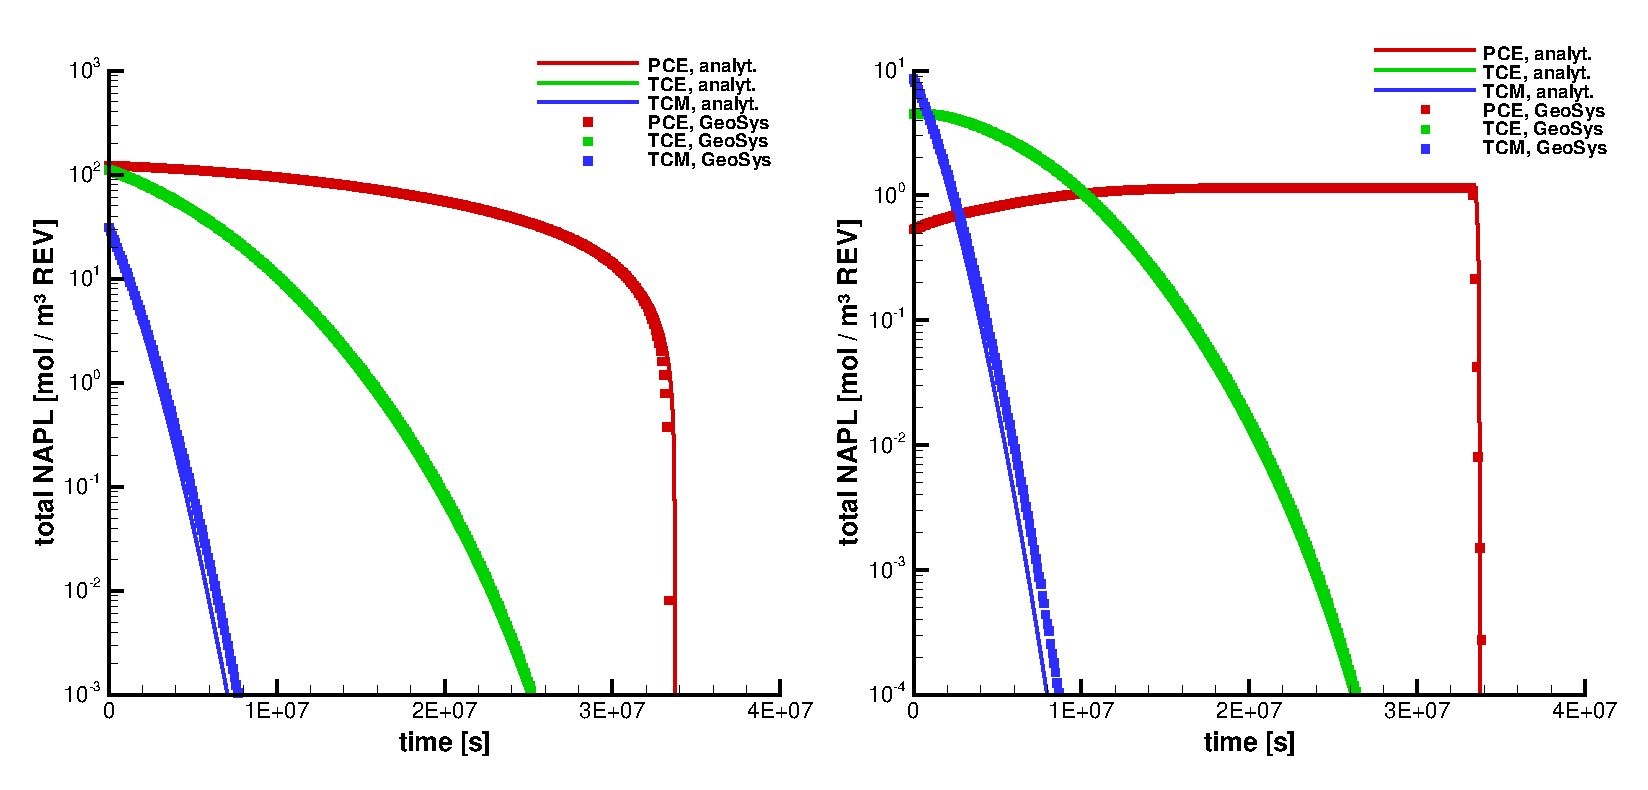
\includegraphics[width=0.9\textwidth]{C/figures/H&K_ASvsGS.eps}
\caption{Total amounts of PCE, TCE and TCM in the NAPL phase (left diagram) and corresponding aqueous phase concentrations at the downgradient source zone margin (right diagram) as functions of time; full lines: analytical solution of Hansen and Kueper (2007), symbols: GeoSys simulation results.}
\label{fig_HKAS_vs_GeoSys}
\end{figure}


\begin{table}[htbp]
\centering
\begin{tabular}{|l|l|l|}
\hline
Benchmark & Type & Path \\
\hline
\texttt{1D\_TPF\_resS\_flow}& HC &  inputfiles$\backslash$benchmarks$\backslash$1D\_NAPL-diss\_flow  \\			
\hline
\texttt{1D\_TPF\_resS\_transport}& HC &  inputfiles$\backslash$benchmarks$\backslash$1D\_NAPL-diss\_transport  \\			 \hline
\texttt{1D\_TPF\_resS\_dissolution}& HC &  inputfiles$\backslash$benchmarks$\backslash$1D\_NAPL-diss\_dissolution \\			 \hline
\end{tabular}
\end{table}
